% !TeX spellcheck = en_US
\documentclass[12pt, a4paper]{article}
\usepackage{comment}
\usepackage{ragged2e}
\usepackage{amsmath}
\usepackage{xcolor}
\usepackage{multirow}
\usepackage{caption}
\usepackage{tikz}
\usepackage{booktabs}
\usepackage{tabu}
\usepackage{placeins}
\usepackage{pdflscape}
\usetikzlibrary{arrows}
\usepackage{hyperref}
\usepackage{multirow}
\usepackage{subcaption}
 \usepackage{pdflscape}



\captionsetup{font=footnotesize,labelfont=footnotesize}

\hypersetup{
    colorlinks=true,
    linkcolor=blue,
    filecolor=blue,      
    urlcolor=blue,
    citecolor=blue
}

\usepackage{natbib}
\usepackage[title]{appendix}

\tikzstyle{startstop} = [rectangle, rounded corners, minimum width=2cm, minimum height=0.75cm,text centered, draw=black, fill=red!30]

\tikzstyle{startstop1} = [rectangle, rounded corners, minimum width=2cm, minimum height=0.75cm,text centered, draw=black, fill=blue!30]

\tikzstyle{startstop2} = [rectangle, rounded corners, minimum width=2cm, minimum height=0.75cm,text centered, draw=black, fill=yellow!30]

\tikzstyle{startstop3} = [rectangle , rounded corners, minimum width=0.5cm, minimum height=0.75cm,text centered,draw=black]


\tikzstyle{io} = [trapezium, trapezium left angle=70, trapezium right angle=110, minimum width=2cm, minimum height=0.75cm, text centered, draw=black, fill=blue!30]



\tikzstyle{process} = [rectangle, minimum width=2cm, minimum height=1cm, text centered, draw=black, fill=green!30]

\tikzstyle{decision} = [diamond, minimum width=0.75cm, minimum height=0.75cm, text centered, draw=black, fill=green!30]

\tikzstyle{arrow} = [thick,->,>=stealth]



\def\sym#1{\ifmmode^{#1}\else\(^{#1}\)\fi}


\renewcommand{\today}{\ifcase \month \or January\or February\or March\or %
April\or May \or June\or July\or August\or September\or October\or November\or %
December\fi, \number \year} 

\title{{How are stocks connected?\\
\small The evidence from emerging market}}
\author{{S.M. Aghajanzadeh\sym{*} \qquad M. Heidari\sym{*} \qquad M. Mohseni\sym{*} }\\
{\sym{*} \footnotesize  Tehran Institute for Advanced Studies, Khatam University, Tehran, Iran}
}

\def\boxit#1{%
  \smash{\color{red}\fboxrule=1pt\relax\fboxsep=2pt\relax%
  \llap{\rlap{\fbox{\vphantom{0}\makebox[#1]{}}}~}}\ignorespaces
}


\usepackage{lipsum}

\linespread{1.2}




\begin{document}
\maketitle


\begin{abstract}

\end{abstract}





\section{Introduction}


\section{Data and Methodology}



\subsection{Data and Sample}


	 \begin{table}[htbp]
        \centering
        \caption{ This table reports summary statistics of ownership features for all the listed firms. At this table by group, we mean business groups.}
        \label{t2-1}
        \resizebox{1\textwidth}{!}
        {
        \begin{tabular}{lrrrrrr}
\toprule
Year &  2014 &  2015 &  2016 &  2017 &  2018 &  2019 \\
\midrule
No. of Firms                        &   365 &   376 &   446 &   552 &   587 &   618 \\
No. of Blockholders                 &  1606 &  1676 &  2099 &  2978 &  3374 &  3416 \\
No. of Groups                       &    38 &    41 &    43 &    44 &    40 &    43 \\
No. of Firms in Groups              &   249 &   268 &   300 &   336 &   346 &   375 \\
Ave. Number of group Members        &     7 &     7 &     7 &     8 &     9 &     9 \\
Ave. ownership of each Blockholders &    18 &    19 &    18 &    17 &    18 &    19 \\
Med. ownership of each Blockholders &     5 &     4 &     4 &     4 &     4 &     4 \\
Ave. Number of Owners               &     7 &     6 &     6 &     7 &     7 &     7 \\
Ave. Block. Ownership               &    77 &    77 &    75 &    76 &    75 &    72 \\
\bottomrule
\end{tabular}

         }
      \end{table}


\subsection{Pair composition} 
 \begin{table}
  \centering
  \caption{ This table reports summary statistics of ownership features for total pairs. At this table by group, we mean business groups.}
  \label{t2-2}
    \resizebox{1\textwidth}{!}
          {
 \begin{tabular}{lrrrrrr}
\toprule
year &   1393 &   1394 &   1395 &   1396 &   1397 &   1398 \\
\midrule
No. of Pairs                          &  20876 &  21187 &  27784 &  41449 &  47234 &  67232 \\
No. of Groups                         &     37 &     40 &     42 &     43 &     39 &     43 \\
No. of Pairs not in Groups            &  11452 &  11192 &  15351 &  26530 &  29182 &  43433 \\
Number of Pairs not in the same Group &   7962 &   8731 &  10971 &  12916 &  15366 &  20745 \\
Number of Pairs in the same Group     &    923 &    955 &   1099 &   1260 &   1536 &   1774 \\
Average Number of Common owner        &      1 &      1 &      1 &      1 &      1 &      1 \\
Med. Number of Common owner           &      1 &      1 &      1 &      1 &      1 &      1 \\
Average Percent of each blockholder   &     19 &     19 &     19 &     19 &     19 &     20 \\
Med. Percent of each blockholder      &     13 &     12 &     12 &     12 &     12 &     14 \\
Average Number of Pairs in one Group  &     31 &     30 &     30 &     34 &     39 &     44 \\
Med. Number of Pairs in one Group     &      8 &     10 &      8 &     10 &      9 &     10 \\
Average Number of Owners              &      5 &      5 &      5 &      5 &      4 &      5 \\
Med. Number of Owners                 &      5 &      5 &      5 &      5 &      4 &      5 \\
Average Block. Ownership              &     73 &     73 &     72 &     70 &     70 &     70 \\
Med. Block. Ownership                 &     73 &     73 &     73 &     71 &     71 &     71 \\
\bottomrule
\end{tabular}

   }
    \end{table}

\begin{figure}[htbp]
	\centering
	\caption{ Three categories for pairs base on being in business groups}
	\label{g2-1}
	
	\normalcolor
	\begin{subfigure}[t]{0.9\linewidth}
		
		\resizebox{0.49\textwidth}{!}{
			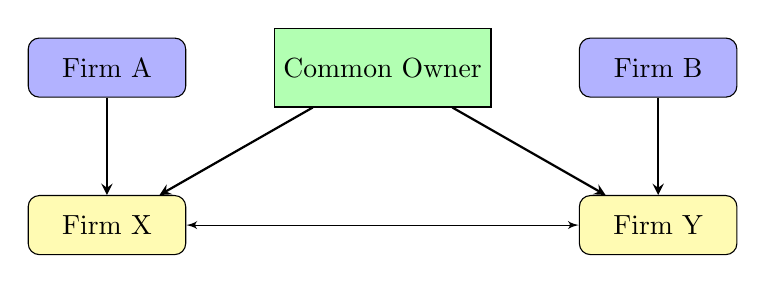
\begin{tikzpicture}[node distance=2cm]
				
				
				
				\node (CH) [process,yshift = -2cm ,xshift=3.5cm] {Common Owner};
				
				\node (end) [startstop1,left of = CH ,xshift=-1.5cm ] {$ \text{Firm A} $};
				
				\node (end2) [startstop1,right of = CH ,yshift=0cm,xshift=1.5cm] {$ \text{Firm B} $};
				
				\node (sur) [startstop2 ,below of = end ,yshift=0cm,xshift=0cm] {$ \text{Firm X} $};
				
				\node (sur2) [startstop2,below of = end2 ,yshift=0cm,xshift=0cm] {$ \text{Firm Y} $};
				
				
				\draw [arrow] (end) --(sur);
				\draw [arrow] (end2) -- (sur2);
				
				
				\draw [arrow] (CH) -- (sur);
				\draw [arrow] (CH) -- (sur2);
				
				\draw [latex'-latex'] (sur) to [bend right =0]  node[sloped, anchor=center, below] {} (sur2);
				
				
			\end{tikzpicture}
		}   
		\hfill
		\resizebox{0.49\textwidth}{!}{
			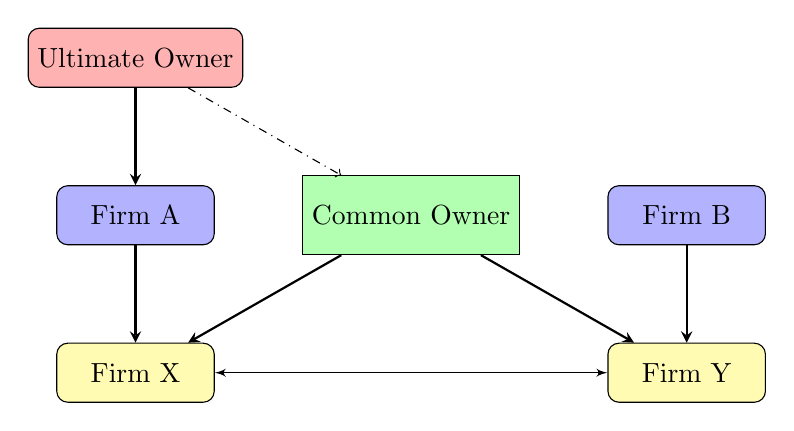
\begin{tikzpicture}[node distance=2cm]
				
				
				\node (start) [startstop] { $ \text{Ultimate Owner} $};
				
				
				\node (CH) [process, below of = start,xshift=3.5cm] {Common Owner};
				
				\node (end) [startstop1,below of = start ] {$ \text{Firm A} $};
				
				\node (end2) [startstop1,right of = CH ,yshift=0cm,xshift=1.5cm] {$ \text{Firm B} $};
				
				\node (sur) [startstop2 ,below of = end ,yshift=0cm,xshift=0cm] {$ \text{Firm X} $};
				
				\node (sur2) [startstop2,below of = end2 ,yshift=0cm,xshift=0cm] {$ \text{Firm Y} $};
				
				
				
				\draw [arrow] (start) --(end);
				
				\draw [arrow] (end) --(sur);
				\draw [arrow] (end2) -- (sur2);
				
				\draw [dash dot,->] (start) -- (CH);
				
				\draw [arrow] (CH) -- (sur);
				\draw [arrow] (CH) -- (sur2);
				
				\draw [latex'-latex'] (sur) to [bend right =0]  node[sloped, anchor=center, below] {} (sur2);
				
				
			\end{tikzpicture}
		}
		\caption{ Pair not in the business group}
	\end{subfigure}
	\bigskip
	\begin{subfigure}[t]{.45\linewidth}
		\centering
		\tiny
		\resizebox{1\textwidth}{!}{
			
			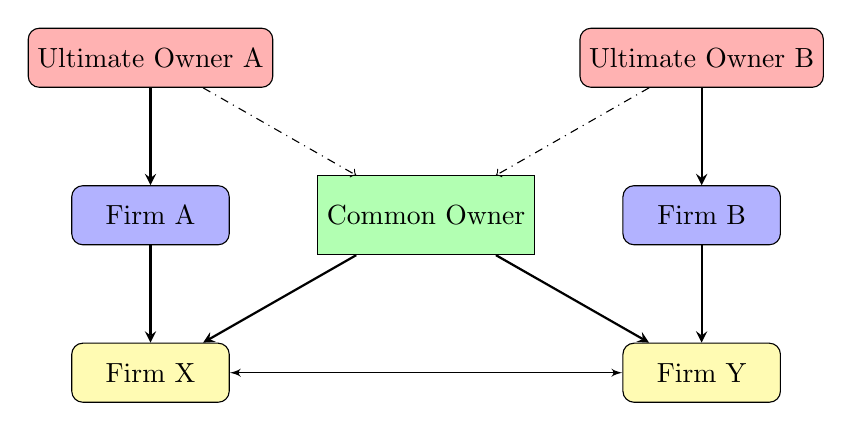
\begin{tikzpicture}[node distance=2cm]
				
				
				\node (start) [startstop] { $ \text{Ultimate Owner A} $};
				\node (start2) [startstop,right of = start,xshift=5cm] {$ \text{Ultimate Owner B} $};
				
				
				\node (CH) [process, below of = start2,xshift=-3.5cm] {Common Owner};
				
				\node (end) [startstop1,below of = start ] {$ \text{Firm A} $};
				
				\node (end2) [startstop1,below of = start2 ,yshift=0cm,xshift=0cm] {$ \text{Firm B} $};
				
				\node (sur) [startstop2 ,below of = end ,yshift=0cm,xshift=0cm] {$ \text{Firm X} $};
				
				\node (sur2) [startstop2,below of = end2 ,yshift=0cm,xshift=0cm] {$ \text{Firm Y} $};
				
				
				
				\draw [arrow] (start) --(end);
				\draw [arrow] (start2) -- (end2);
				
				\draw [arrow] (end) --(sur);
				\draw [arrow] (end2) -- (sur2);
				
				\draw [dash dot,->] (start) -- (CH);
				\draw [dash dot,->] (start2) -- (CH);
				
				\draw [arrow] (CH) -- (sur);
				\draw [arrow] (CH) -- (sur2);
				
				\draw [latex'-latex'] (sur) to [bend right =0]  node[sloped, anchor=center, below] {} (sur2);
				
				
			\end{tikzpicture}
		}   
		\caption{ Pair in two distinct business group}
	\end{subfigure}
	\begin{subfigure}[t]{.45\linewidth}
		\centering
		\tiny
		\resizebox{1\textwidth}{!}{
			
			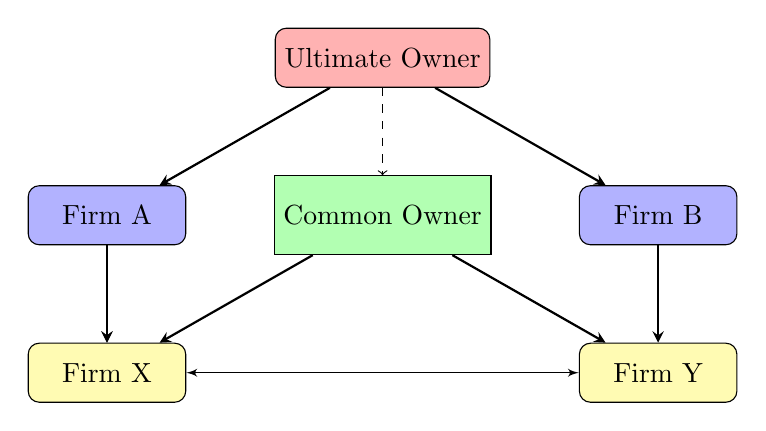
\begin{tikzpicture}[node distance=2cm]
				
				
				\node (start) [startstop] {Ultimate Owner};
				
				
				
				\node (end) [startstop1,below of = start , yshift=0cm , xshift=-3.5cm ] {$ \text{Firm A} $};
				\node (end2) [startstop1,below of = start , yshift=0cm , xshift=3.5cm ] {$ \text{Firm B} $};
				
				
				
				\node (sur) [startstop2 ,below of = end ,yshift=0cm,xshift=0cm] {$ \text{Firm X} $};
				
				
				\node (sur2) [startstop2 ,below of = end2 ,yshift=0cm,xshift=0cm] {$ \text{Firm Y} $};
				
				
				\node (CH) [process, below of = start ,xshift=0] {Common Owner};
				
				
				\draw [arrow] (start) --(end);
				\draw [arrow] (end) --(sur);
				
				\draw [arrow] (start) --(end2);
				
				\draw [arrow] (end) --(sur);
				\draw [arrow] (end2) -- (sur2);
				
				
				\draw [arrow] (CH) -- (sur);
				\draw [arrow] (CH) -- (sur2);
				\draw [dashed ,->] (start) --(CH);
				
				\draw [latex'-latex'] (sur) to [bend right =0]  node[sloped, anchor=center, below] {} (sur2);
				
				
			\end{tikzpicture}
		} 
		
		\caption{ Pair in the same business group}
	\end{subfigure}
	
	
	
\end{figure}  


  \FloatBarrier
  
  
  
\subsection{Stock Return co-movement}
\label{comovement}

 \begin{table}[htbp]
        \centering
        \caption{\footnotesize This table reports distribution of calculated correlation base on different models.}
        \label{tCorr}
        \resizebox{1\textwidth}{!}
        {
        \begin{tabular}{lrrrrr}
\toprule
{} &   mean &    std &  min &  median &  max \\
\midrule
 CAPM + Industry    &  0.018 &  0.205 & -1.0 &   0.018 &  1.0 \\
4 Factor            &  0.031 &  0.206 & -1.0 &   0.027 &  1.0 \\
4 Factor + Industry &  0.014 &  0.204 & -1.0 &   0.012 &  1.0 \\
\bottomrule
\end{tabular}

         }
      \end{table}
      

\FloatBarrier


\subsection{Controls}

\begin{table}[htbp]
\caption{\scriptsize This table reports the number of pairs in the same industry and business group.}
\label{SameGroupIndustry}
               \centering \scriptsize
         {

    \begin{tabular}{lcc}\hline\hline
    {Type of Pairs} & {Yes} &{No} \\
    \hline
    \addlinespace
    {SameIndustry} & 1760  & 16739 \\
          & \tiny(10\%) & \tiny (90\%) \\
          \addlinespace
{SameGroup} & 1118  & 17381 \\
          & \tiny(6\%) & \tiny (94\%) \\
          \addlinespace
{SameGroup \& SameIndustry} & 492  & 18007 \\
          & \tiny(3\%) & \tiny (97\%) \\    
                
          \hline\hline
    \end{tabular}%
                 }
             \end{table}
 \begin{table}[htbp]
 \caption{\scriptsize This table shows the summary statistics of specified controls in empirical studies.}
 \label{ControlsSummary}
               \centering 
               \scriptsize
                \resizebox{\textwidth}{!}  {
    \begin{tabular}{lrrrrrrr}\hline\hline
          & \multicolumn{1}{l}{mean} & \multicolumn{1}{l}{std} & \multicolumn{1}{l}{min} & 25\%  & 50\%  & 75\%  & \multicolumn{1}{l}{max} \\
          \hline
          
          SameIndustry & 0.10  & 0.29  & 0.00  & 0.00  & 0.00  & 0.00  & 1.00 \\
          SameGroup & 0.06  & 0.23  & 0.00  & 0.00  & 0.00  & 0.00  & 1.00 \\
          Size1 & 0.72  & 0.21  & 0.01  & 0.58  & 0.78  & 0.91  & 1.00 \\
          Size2 & 0.43  & 0.25  & 0.00  & 0.23  & 0.42  & 0.62  & 0.99 \\
          SameSize & -0.29 & 0.21  & -0.97 & -0.42 & -0.24 & -0.12 & 0.00 \\
          BookToMarket1 & 0.53  & 0.26  & 0.00  & 0.34  & 0.54  & 0.73  & 1.00 \\
          BookToMarket2 & 0.52  & 0.24  & 0.00  & 0.34  & 0.52  & 0.71  & 1.00 \\
          SameBookToMarket & -0.30 & 0.19  & -0.99 & -0.42 & -0.26 & -0.15 & 0.00 \\
          MonthlyCrossOwnership & 0.01  & 0.05  & 0.00  & 0.00  & 0.00  & 0.00  & 0.96 \\
          
    
    \hline\hline
            \end{tabular}
                 }
             \end{table}
         
         
 


\FloatBarrier

\subsection{Measurement of common-ownership}

\begin{table}[htbp]
	\centering
	\scriptsize
	\caption{ This table summarizes common ownership measurements in the literature.}
	\label{maasurmentsSummary}
	\resizebox{\textwidth}{!}{
		\begin{tabular}{cllc}
	\hline\hline
	\multicolumn{1}{c}{Group}      & \multicolumn{1}{c}{Paper} & \multicolumn{1}{c}{measurment} & \multicolumn{1}{c}{Flaws} \\
	\hline\hline
	\addlinespace
	\multicolumn{1}{c}{\multirow{5}[2]{*}{Model Based}} &  \cite{harford2011institutional}     &  \scriptsize  $
	\sum_{i\in I^{A,B}}\frac{\alpha_{i,B}}{\alpha_{i,A} + \alpha_{i,B}}     $     & Bi-directional \\
	\addlinespace 
	&  \cite{azar2018anticompetitive}     &  $   \sum_{j} \sum_k s_j s_k \frac{\sum_i \mu_{ij} \nu_{ik}}{\sum_i \mu_{ij} \nu_{ij}}   $     & Industry level \\
	\addlinespace
	&  \cite{gilje2020s}     &    $ \sum_{i = 1}^{I} \alpha_{i,A}g(\beta_{i,A})\alpha_{i,B}    $   & Bi-directional  \\
	\midrule
	\addlinespace 
	\multicolumn{1}{c}{\multirow{7}[5]{*}{Ad hoc}} & \cite{he2017product};      &  \multirow{2}{*}{$ \sum_{i\in I^{A,B}} 1 $}     & invariant to the level   \\
	& \cite{he2019internalizing} & & of ‌common ownership \\
	\addlinespace
	&  \cite{newham2018common}     &   $ \sum_{i\in I^{A,B}} min\{\alpha_{i,A},\alpha_{i,B}\} $    & ? \\
	\addlinespace
	& \multirow{2}{*}{   \cite{AntonPolk} }  &  \multirow{2}{*}{ $ \sum_{i\in I^{A,B}} \alpha_{i,A}\frac{\bar{\nu}_A}{\bar{\nu}_A +\bar{\nu}_B } + \alpha_{i,B}\frac{\bar{\nu}_B}{\bar{\nu}_A +\bar{\nu}_B }  $ }   &  Invariant to the  \\
	& & & decomposition of ownership \\
	\addlinespace
	& \cite{freeman2019effects}; & \multirow{2}{*}{ $ \sum_{i\in I^{A,B}} \alpha_{i,A} \times \sum_{i\in I^{A,B}} \alpha_{i,B} $ }&?\\
	&  \cite{hansen1996externalities} & & ?\\
	\hline\hline
\end{tabular}
	}
\end{table}



\subsubsection{Modified Anton's measure}


				\begin{figure}[htbp]
				\centering
				\caption{ Numeric example 1} 
				\label{gExample1}
				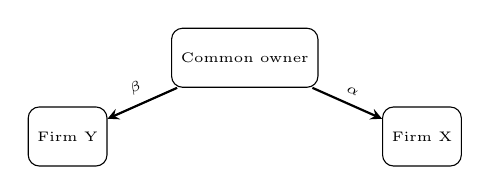
\begin{tikzpicture}[node distance=1cm]
					
					\node (Firm) [startstop3] {\tiny Firm X};
					\node (Firm2) [startstop3,right of = Firm  , xshift=-5.5cm ] {\tiny Firm Y};
					\node (Owner) [startstop3,right of = Firm , yshift=1cm , xshift=-3.25cm ] {\tiny Common owner };
					
					
					\draw[arrow] (Owner) -- node[sloped, anchor=center, above] {\tiny $ \alpha $} (Firm) ;
					
					\draw[arrow] (Owner) -- node[sloped, anchor=center, above] {\tiny $ \beta $} (Firm2) ;
					%
					%\node() at (3,0)
					%    {$ \alpha + \beta = 100 $}; 
				\end{tikzpicture}
			\end{figure}\bigskip

\begin{figure}[htbp]
	\caption{ Comparison of three measure for common ownership}
	\label{example1Results}
	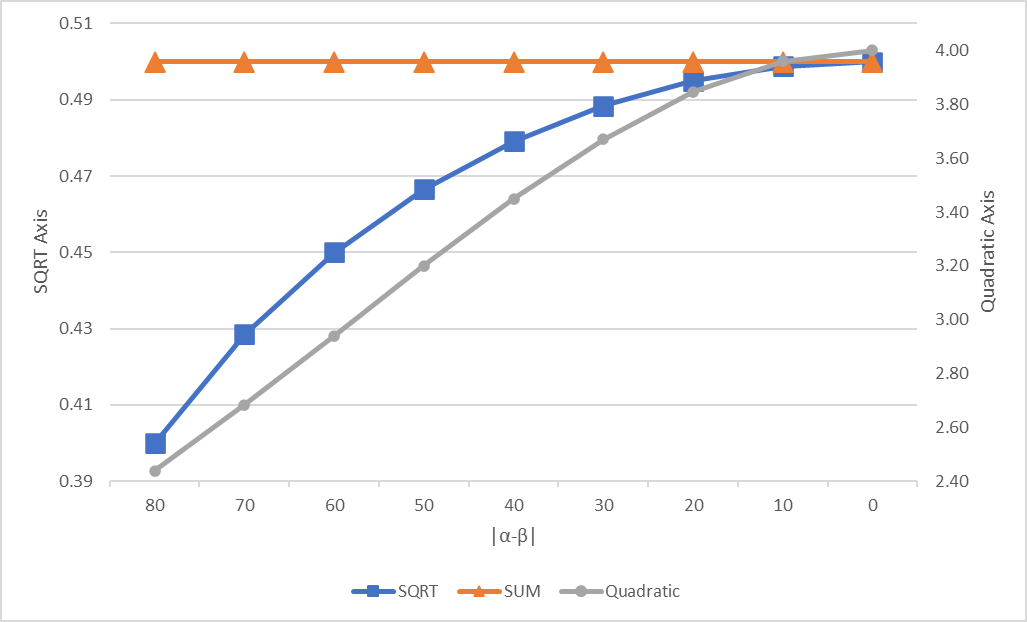
\includegraphics[width=0.47\linewidth]{1.png}
	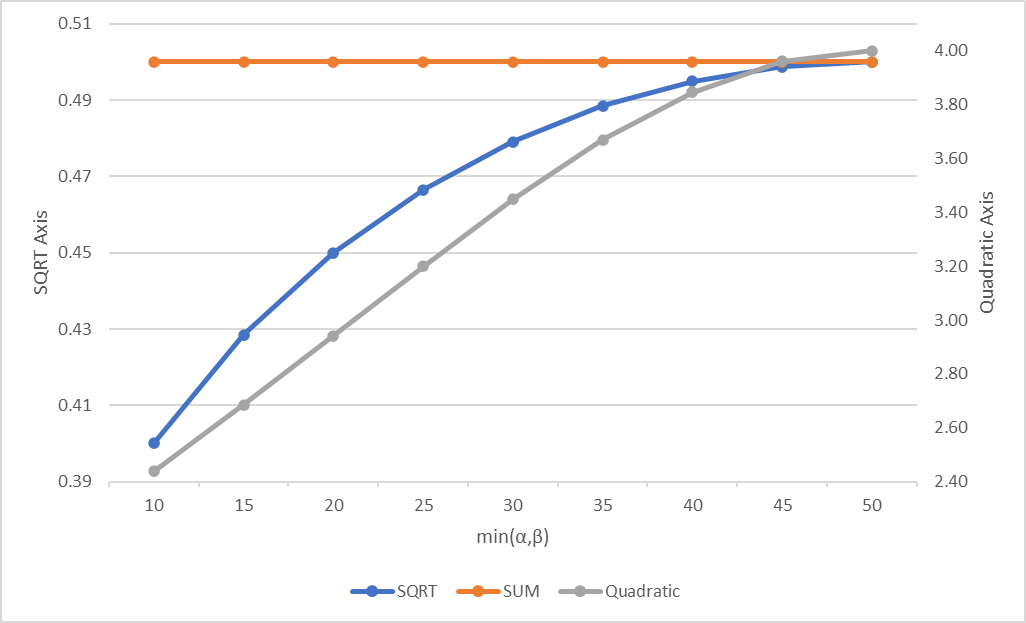
\includegraphics[width=0.47\linewidth]{2.png}
\end{figure}


			\begin{figure}[htbp]  \centering
				\caption{ Numeric example 2}
				\label{gExample2}
				\centering
				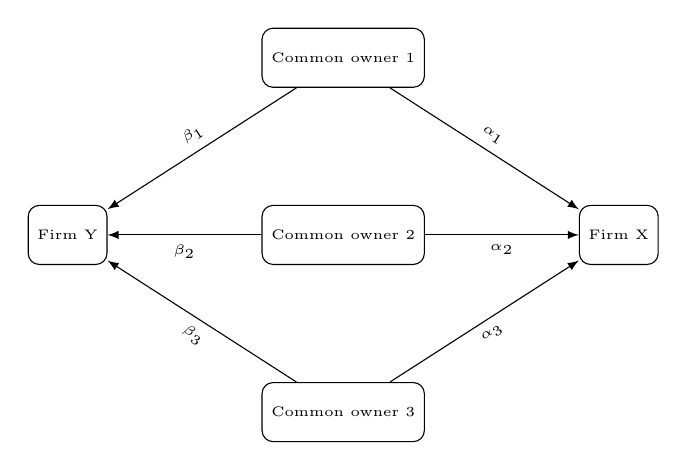
\begin{tikzpicture}[node distance=1cm]
					
					
					\node (Firm) [startstop3] {\tiny Firm X};
					\node (Firm2) [startstop3,right of = Firm , yshift=0cm , xshift=-8cm ] {\tiny Firm Y};
					
					\node (Owner) [startstop3,above of = Firm , yshift=1.25cm , xshift=-3.5cm ] {\tiny Common owner 1 };
					
					
					\node (Owner2) [startstop3,right of = Firm , yshift= 0 , xshift=-4.5cm ] {\tiny Common owner 2 };
					
					\node (Owner3) [startstop3,below of = Firm , yshift=-1.25cm , xshift=-3.5cm ] {\tiny Common owner 3 };
					
					
					
					
					
					\draw [-latex] (Owner) to [bend right =0]  node[sloped, anchor=center, above] {\tiny $ \beta_1 $} (Firm2);
					
					\draw [-latex] (Owner) to [bend left =0]  node[sloped, anchor=center, above] {\tiny $ \alpha_1 $} (Firm);
					
					
					
					\draw [-latex] (Owner2) to [bend right =0]  node[sloped, anchor=center, below] {\tiny $ \beta_2 $} (Firm2);
					
					\draw [-latex] (Owner2) to [bend left =0]  node[sloped, anchor=center, below] {\tiny $ \alpha_2 $} (Firm);
					
					
					
					\draw [-latex] (Owner3) to [bend left =0]  node[sloped, anchor=center, below] {\tiny$ \beta_3 $} (Firm2);
					
					\draw [-latex] (Owner3) to [bend right =0]  node[sloped, anchor=center, below] {\tiny $ \alpha_3 $} (Firm);
					
					
					
				\end{tikzpicture}
			\end{figure}
			\begin{table}[htbp]
				\centering
				\caption{ text}
				\label{Example2}
				\resizebox{1\textwidth}{!}
				{
					    \begin{tabular}{cccccccc}
    \hline\hline
        Ownership  & Type I & Type II & Type III & Type IV & Type V & Type VI & Type VII \\
          \hline
    $ \alpha_1 $    & 1/3 &20      &  10   & 20    & 10    & 5     & 1  \\
    $ \beta_1 $    & 1/3  & 10    & 10   & 20    & 10    & 5     & 1  \\
    $ \alpha_2 $    & 1/3  & 10    & 80    & 20    & 10    & 5     & 1 \\
    $ \beta_2 $    & 1/3  & 20    & 80    & 20    & 10    & 5     & 1  \\
    $ \alpha_3 $    & 1/3  & 70    & 10    & 20    & 10    & 5     & 1 \\
    $ \beta_3 $    & 1/3  & 70    & 10   & 20    & 10    & 5     & 1  \\
    \hline
    SQRT  & 3     &  2.56  & 2.33 & 1.8   & 0.9   & 0.45  & 0.09 \\
    SUM   & 1     & 1     & 1     & 0.6   & 0.3   & 0.15  & 0.03 \\
    Quadratic & 3     & 1.85  & 1.52  & 8.33  & 33.33 & 133.33 & 3333.33 \\
 
    \hline\hline
    \end{tabular}%
				}
			\end{table}
			\begin{figure}[htbp]
				\centering
				\caption{ SQRT measure for fixed aggregate ownership on different relative market cap ratios}
				\label{sqrtMarket}
				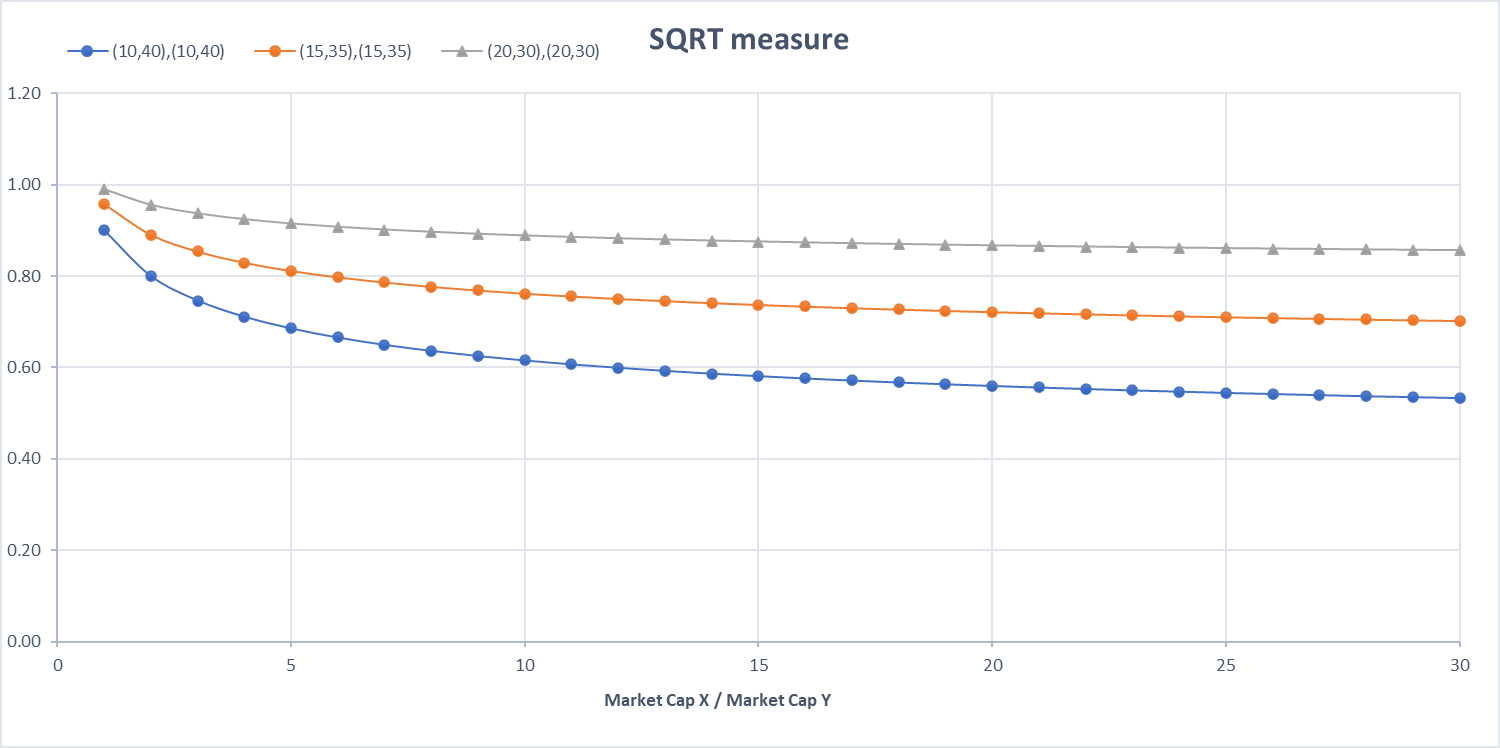
\includegraphics[width=0.85\linewidth]{3.png}
			\end{figure}
			\begin{figure}[htbp]
				\centering
				\caption{ Sum measure for fixed aggregate ownership on different relative market cap ratios}
				\label{sumMarket}
				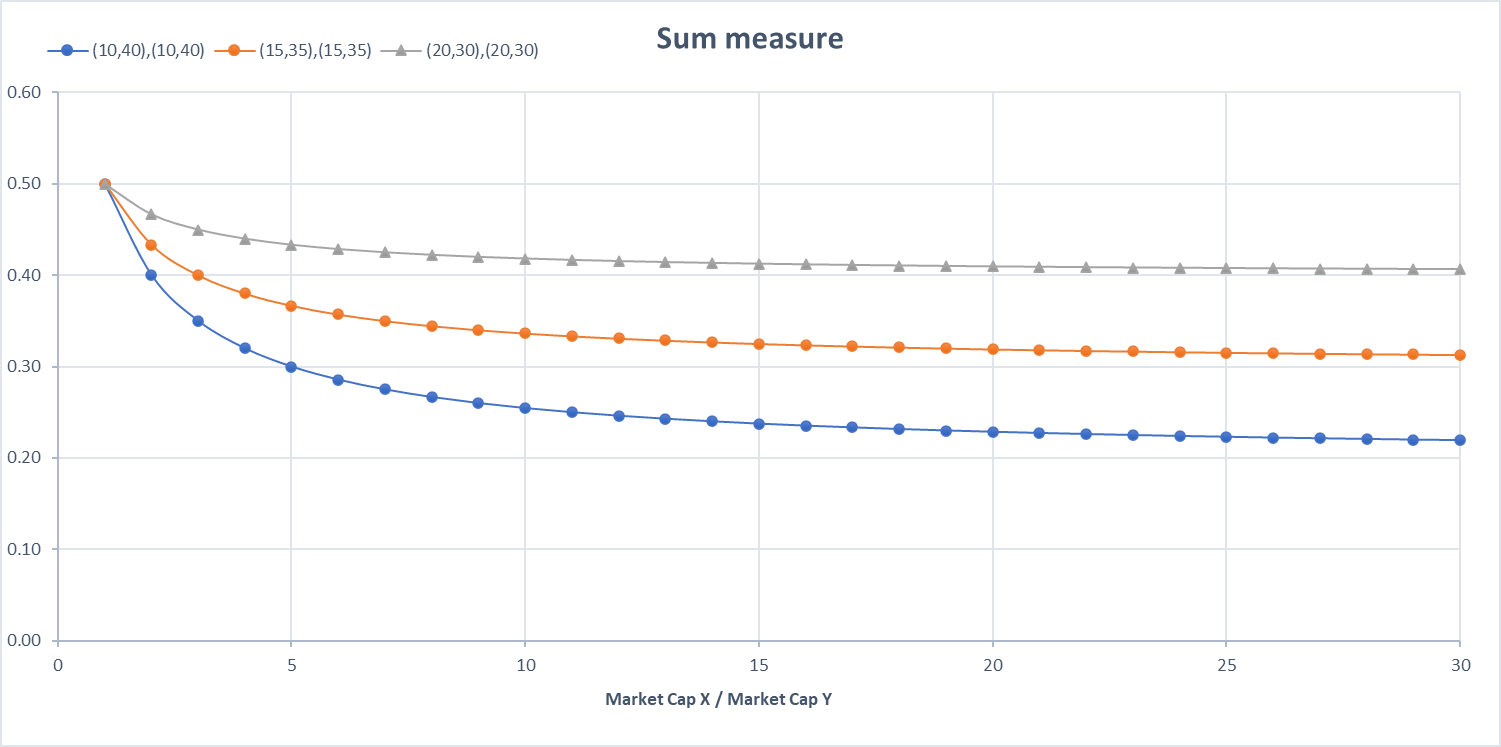
\includegraphics[width=0.85\linewidth]{4.png}
			\end{figure}
			\begin{table}[htbp]
						\centering
						\caption{text }
						\label{marketcap}
						\resizebox{!}{!}
						{
							          \scriptsize
    \begin{tabular}{ccccccc}
    \hline\hline
  & \multicolumn{6}{c}{\tiny($ \alpha_1 $,$ \beta_1 $),($ \alpha_2 $,$ \beta_2 $) }\\ \cmidrule(lr){2-7}
               & \multicolumn{2}{c}{\tiny(10,40),(10,40)} & \multicolumn{2}{c}{\tiny(15,35),(15,35)} & \multicolumn{2}{c}{\tiny(20,30),(20,30)} \\ \cmidrule(lr){2-3}\cmidrule(lr){4-5}\cmidrule(lr){6-7}
    \tiny $ \frac{\text{MarketCap}_x}{\text{MarketCap}_y} $     &\tiny SQRT  & \tiny SUM   &\tiny SQRT  &\tiny SUM   &\tiny SQRT  &\tiny SUM \\ 
     \hline\addlinespace

         1     & 0.90  & 0.50  & 0.96  & 0.50  & 0.99  & 0.50 \\
         2     & 0.80  & 0.40  & 0.89  & 0.43  & 0.96  & 0.47 \\
         3     & 0.75  & 0.35  & 0.85  & 0.40  & 0.94  & 0.45 \\
         4     & 0.71  & 0.32  & 0.83  & 0.38  & 0.92  & 0.44 \\
         5     & 0.69  & 0.30  & 0.81  & 0.37  & 0.91  & 0.43 \\
         6     & 0.67  & 0.29  & 0.80  & 0.36  & 0.91  & 0.43 \\
         7     & 0.65  & 0.28  & 0.79  & 0.35  & 0.90  & 0.43 \\
         8     & 0.64  & 0.27  & 0.78  & 0.34  & 0.90  & 0.42 \\
         9     & 0.63  & 0.26  & 0.77  & 0.34  & 0.89  & 0.42 \\
         10    & 0.62  & 0.25  & 0.76  & 0.34  & 0.89  & 0.42 \\
     
    \hline\hline
    \end{tabular}
						}
				\end{table}
		
		








\begin{table}[htbp]
	\centering
	\caption{ text}
	\label{measureResults}
	\resizebox{1\textwidth}{!}
	{
		\begin{tabular}{lrrrrrrrrrr}
\toprule
\multirow{2}{*}{Subset}& \multicolumn{5}{c}{MFCAP} & \multicolumn{5}{c}{FCAP} \\
\cmidrule(lr){2-6} \cmidrule(lr){7-11}
&       mean &    std &    min & median &    max &         mean &    std &    min & median &    max \\
\midrule
All               &  0.15 &  0.24 &  0.00 &   0.06 &  4.62 &  0.12 &  0.16 &  0.0 &   0.05 &  0.97 \\
Same Group        &  0.47 &  0.41 &  0.00 &   0.41 &  4.04 &  0.38 &  0.25 &  0.0 &   0.37 &  0.97 \\
Not Same Group    &  0.10 &  0.16 &  0.00 &   0.04 &  2.90 &  0.08 &  0.11 &  0.0 &   0.04 &  0.97 \\
Same Industry     &  0.34 &  0.41 &  0.01 &   0.18 &  4.04 &  0.25 &  0.24 &  0.0 &   0.16 &  0.96 \\
Not Same Industry &  0.12 &  0.19 &  0.00 &   0.05 &  4.62 &  0.10 &  0.14 &  0.0 &   0.05 &  0.97 \\
\bottomrule
\end{tabular}

	}
\end{table}










\FloatBarrier



\subsection{Overview of Business Groups in Tehran Stock Exchange} \label{BGDef}


		\begin{figure}[htbp]
			\caption{}
			\label{sameIndustryinBG}
			\centering
			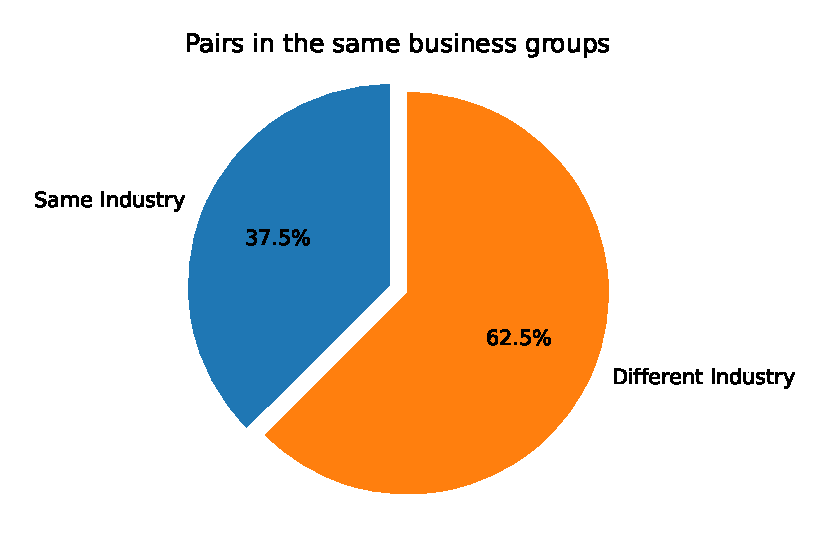
\includegraphics[width=0.48\linewidth]{Output/sameIndustryinBG.eps}
			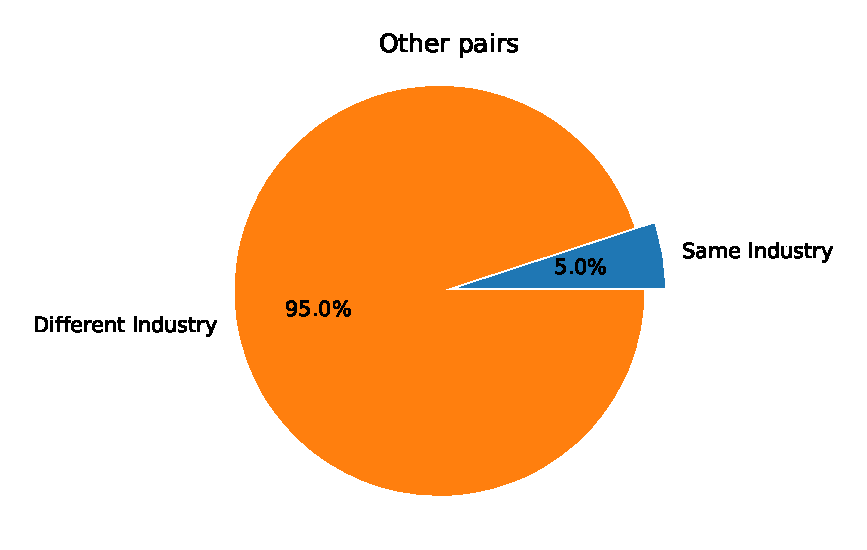
\includegraphics[width=0.48\linewidth]{Output/sameIndustryNoinBG.eps}
		\end{figure}

	\begin{figure}[htbp]
		\caption{}
		\label{BGSummary}
		\centering
		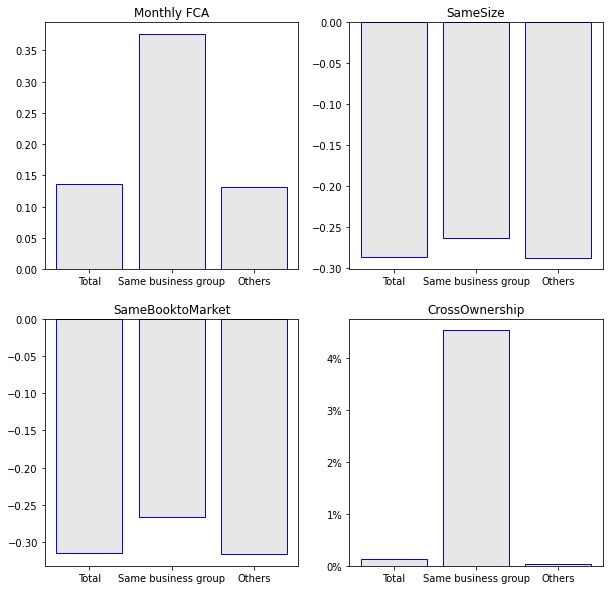
\includegraphics[width=0.85\linewidth]{Output/BGSummary.eps}
	\end{figure}



\FloatBarrier




\section{Results}



\subsection{Forecasting Co-movement}
\label{Forecasting Co-movement}


	 \begin{figure}[htbp]
		\centering  
		\centering
		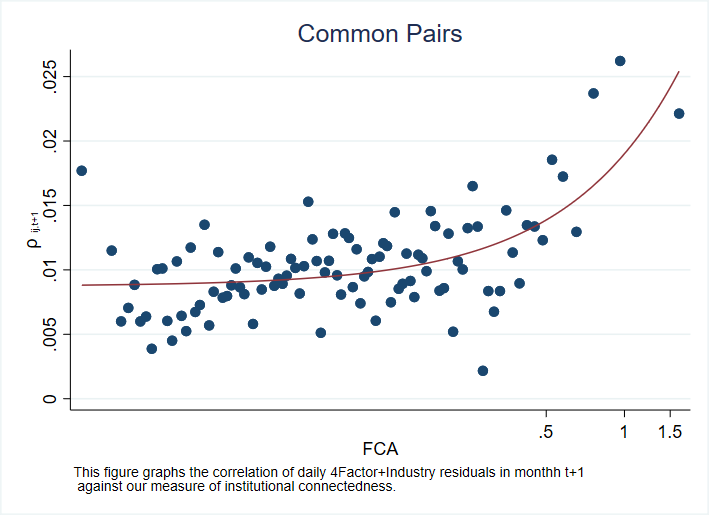
\includegraphics[width=0.7\linewidth]{"Output/mcorr50.eps"} 
		\caption{Future monthly correlation for different level of common ownership at this period }
		\label{mcorr50}
	\end{figure}
	

 \begin{landscape}

	{\begin{table}[htbp]
%	\centering
	\caption{Connected Co-movement}
	\label{mresult2}
%	\resizebox{1\textwidth}{!}{
		{
\def\sym#1{\ifmmode^{#1}\else\(^{#1}\)\fi}
\begin{tabular}{l*{7}{c}}
\hline\hline
                &\multicolumn{7}{c}{Dependent Variable: Future Monthly Correlation of 4F+Industry Residuals}                                         \\\cmidrule(lr){2-8}
                &\multicolumn{1}{c}{(1)}         &\multicolumn{1}{c}{(2)}         &\multicolumn{1}{c}{(3)}         &\multicolumn{1}{c}{(4)}         &\multicolumn{1}{c}{(5)}         &\multicolumn{1}{c}{(6)}         &\multicolumn{1}{c}{(7)}         \\
\hline
Same Group      &   0.0138\sym{***}&   0.0128\sym{***}&                  &                  &  0.00978\sym{***}&  0.00458         &  0.00356         \\
                &   (5.76)         &   (6.29)         &                  &                  &   (4.29)         &   (1.43)         &   (1.11)         \\
[1em]
$ \text{FCA*} $ &                  &                  &  0.00405\sym{***}&  0.00375\sym{***}&  0.00296\sym{***}&  0.00258\sym{***}&  0.00273\sym{***}\\
                &                  &                  &   (4.94)         &   (5.12)         &   (3.77)         &   (3.53)         &   (3.51)         \\
[1em]
 $ (\text{FCA}^*) \times {\text{SameGroup} }  $ &                  &                  &                  &                  &                  &  0.00524\sym{**} &  0.00517\sym{**} \\
                &                  &                  &                  &                  &                  &   (3.21)         &   (3.18)         \\
\hline
Observations    &   388492         &   388492         &   388492         &   388492         &   388492         &   388492         &   388492         \\
Group Effect    &       No         &       No         &       No         &       No         &       No         &       No         &      Yes         \\
Controls        &       No         &      Yes         &       No         &      Yes         &      Yes         &      Yes         &      Yes         \\
$ R^2 $         & 0.000404         &  0.00200         & 0.000423         &  0.00201         &  0.00229         &  0.00245         &  0.00875         \\
\hline\hline
\multicolumn{8}{l}{\footnotesize \textit{t} statistics in parentheses}\\
\multicolumn{8}{l}{\footnotesize \sym{*} \(p<0.05\), \sym{**} \(p<0.01\), \sym{***} \(p<0.001\)}\\
\end{tabular}
}

%	}
\end{table}}
 \end{landscape}
\FloatBarrier



\subsection{High level of common ownership}

	\begin{figure}[htbp]
		\centering  
		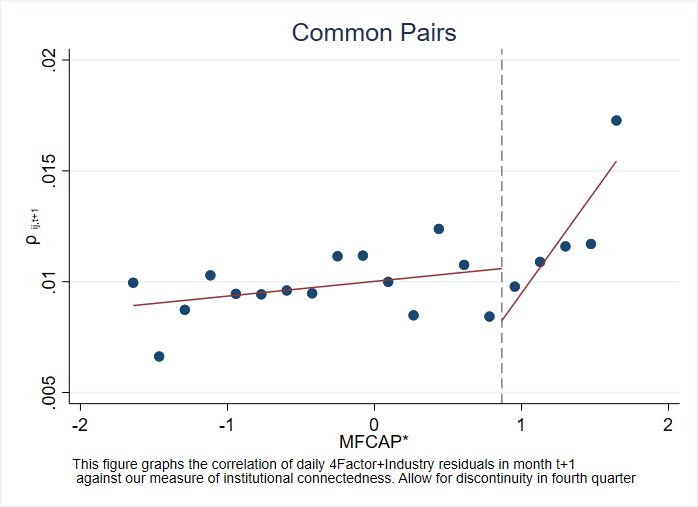
\includegraphics[width=0.6\linewidth]{"Output/Qmcorr5lrd.eps"}
		\caption{text}
		\label{Qmcorr5lrd}
	\end{figure}
	\begin{figure}[htbp]
		\centering  
		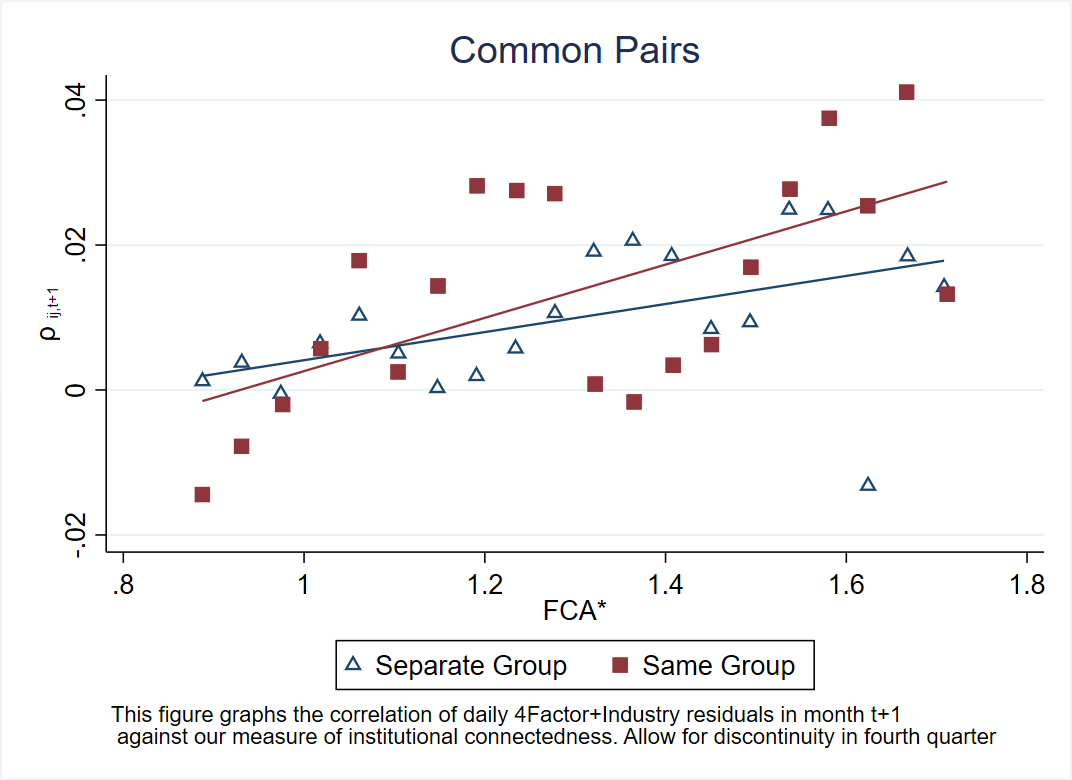
\includegraphics[width=0.45\linewidth]{"Output/Qmcorr5lrdbgsubsample.eps"}
		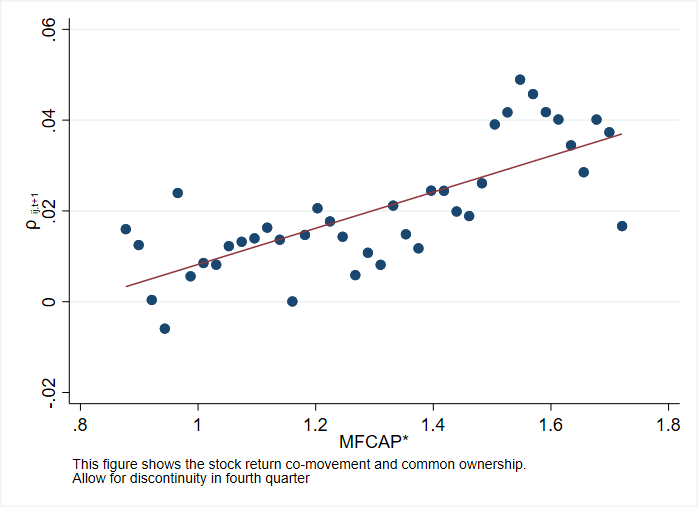
\includegraphics[width=0.45\linewidth]{"Output/Qmcorr5subsample.eps"}
		\caption{text}
		\label{Qmcorr5subsample}
	\end{figure}
 \begin{table}[htbp]
	 	\centering
	 	\caption{\scriptsize Estimation results for high level of common ownership}
	 	\label{QTimemresult2subsample}
	 	\resizebox{0.75\textwidth}{!}{
	 		{
\def\sym#1{\ifmmode^{#1}\else\(^{#1}\)\fi}
\begin{tabular}{l*{7}{c}}
\hline\hline
                &\multicolumn{7}{c}{Dependent Variable:  Future Pairs's Comovement}                                                                  \\\cmidrule(lr){2-8}
                &\multicolumn{1}{c}{(1)}         &\multicolumn{1}{c}{(2)}         &\multicolumn{1}{c}{(3)}         &\multicolumn{1}{c}{(4)}         &\multicolumn{1}{c}{(5)}         &\multicolumn{1}{c}{(6)}         &\multicolumn{1}{c}{(7)}         \\
\hline
SameGroup       &   0.0254\sym{***}&                  &   0.0249\sym{***}&                  &                  &  0.00477         &  0.00252         \\
                &   (8.45)         &                  &   (8.21)         &                  &                  &   (1.32)         &   (0.66)         \\
[1em]
$ (\text{MFCAP} > \text{Larger than 75th Percentile}) $ &                  &  0.00660\sym{***}& 0.000777         &   0.0230\sym{***}& -0.00258\sym{*}  & -0.00157         &-0.000513         \\
                &                  &   (5.48)         &   (0.73)         &   (7.09)         &  (-2.00)         &  (-1.29)         &  (-0.46)         \\
[1em]
 $ (\text{MFCAP} > Q3[\text{MFCAP}]) \times {\text{SameGroup}} $ &                  &                  &                  &                  &                  &   0.0248\sym{***}&   0.0237\sym{***}\\
                &                  &                  &                  &                  &                  &   (7.24)         &   (7.34)         \\
\hline
Sub-sample      &      All         &      All         &      All         &SameGroup         &   Others         &      All         &      All         \\
Controls        &      Yes         &      Yes         &      Yes         &      Yes         &      Yes         &      Yes         &      Yes         \\
Business Group FE&       No         &       No         &       No         &       No         &       No         &       No         &      Yes         \\
Observations    &   389591         &   389591         &   389591         &    47076         &   342515         &   389591         &   389591         \\
\hline\hline
\multicolumn{8}{l}{\footnotesize \textit{t} statistics in parentheses}\\
\multicolumn{8}{l}{\footnotesize \sym{*} \(p<0.05\), \sym{**} \(p<0.01\), \sym{***} \(p<0.001\)}\\
\end{tabular}
}

	 	}
	 \end{table}

	
			\begin{figure}[htbp]
				\centering  
				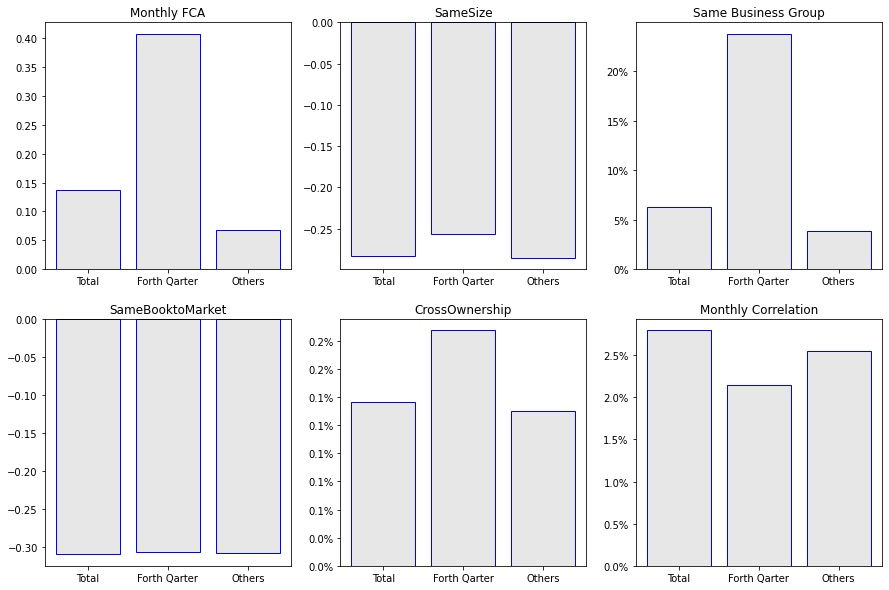
\includegraphics[width=0.75\linewidth]{"Output/QarterSummary.eps"}
				\caption{Pairs' characteristics for the pairs with high level of common ownership}
				\label{QarterSummary}
			\end{figure}


\FloatBarrier

\subsection{All Pairs}

\begin{landscape}

	\begin{table}[htbp]
		%	\centering
		\caption{Non-connected Co-movement}
		\label{AllPairs}
		\resizebox{1.7\textwidth}{!}{
			{
\def\sym#1{\ifmmode^{#1}\else\(^{#1}\)\fi}
\begin{tabular}{l*{7}{c}}
\hline\hline
                &\multicolumn{7}{c}{Dependent Variable: Future Pairs' co-movement}                                                                   \\\cmidrule(lr){2-8}
                &\multicolumn{1}{c}{(1)}         &\multicolumn{1}{c}{(2)}         &\multicolumn{1}{c}{(3)}         &\multicolumn{1}{c}{(4)}         &\multicolumn{1}{c}{(5)}         &\multicolumn{1}{c}{(6)}         &\multicolumn{1}{c}{(7)}         \\
\hline
SameGroup       &   0.0156\sym{***}&                  &   0.0158\sym{***}&                  &                  &   0.0138\sym{***}&   0.0131\sym{***}\\
                &   (9.84)         &                  &  (10.22)         &                  &                  &   (8.27)         &   (7.68)         \\
[1em]
$ \text{MFCAP*}  $&                  &-0.0000723         &-0.000277         &  0.00169         &-0.000322\sym{*}  &-0.000390\sym{**} &-0.000427\sym{*}  \\
                &                  &  (-0.44)         &  (-1.80)         &   (1.42)         &  (-2.19)         &  (-2.70)         &  (-2.29)         \\
[1em]
 $ (\text{MFCAP}^*) \times {\text{SameGroup} }  $ &                  &                  &                  &                  &                  &  0.00313\sym{**} &  0.00364\sym{**} \\
                &                  &                  &                  &                  &                  &   (2.80)         &   (3.34)         \\
\hline
Controls        &      Yes         &      Yes         &      Yes         &      Yes         &      Yes         &      Yes         &      Yes         \\
Sub-Sample      &    Total         &    Total         &    Total         &SameGroups         &   Others         &    Total         &    Total         \\
Business Group FE&       No         &       No         &       No         &       No         &       No         &       No         &      Yes         \\
Observations    &  6018646         &  6018646         &  6018646         &   114526         &  5904120         &  6018646         &  6018646         \\
\hline\hline
\multicolumn{8}{l}{\footnotesize \textit{t} statistics in parentheses}\\
\multicolumn{8}{l}{\footnotesize \sym{*} \(p<0.05\), \sym{**} \(p<0.01\), \sym{***} \(p<0.001\)}\\
\end{tabular}
}

		}
	\end{table}
\end{landscape}


\FloatBarrier




\subsection{Size effect}

	\begin{figure}[htbp]
		\centering  
		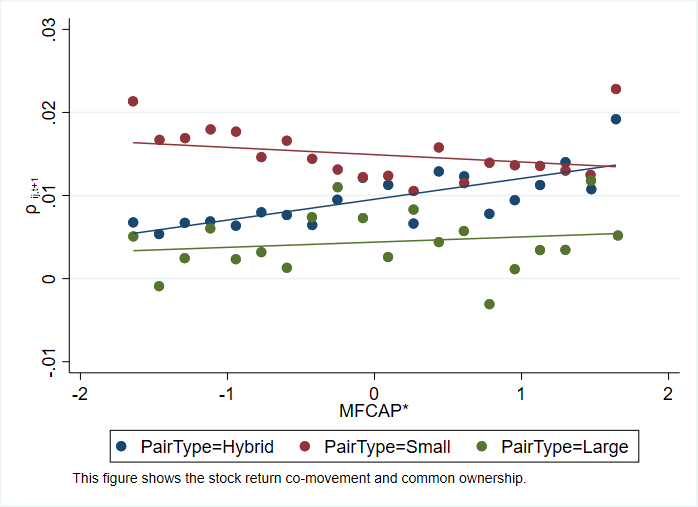
\includegraphics[width=0.7\linewidth]{"Output/mcorrPairType.eps"}
		\caption{text}
		\label{mcorrPairType}
	\end{figure}

		\begin{table}[htbp]
				\centering
				\caption{text}
				\label{Qmresult4}
				\resizebox{1\textwidth}{!}{
					{
\def\sym#1{\ifmmode^{#1}\else\(^{#1}\)\fi}
\begin{tabular}{l*{8}{c}}
\hline\hline
                &\multicolumn{8}{c}{Dependent Variable: Future Monthly Correlation of 4F+Ind. Res.}                                                                     \\\cmidrule(lr){2-9}
                &\multicolumn{1}{c}{(1)}         &\multicolumn{1}{c}{(2)}         &\multicolumn{1}{c}{(3)}         &\multicolumn{1}{c}{(4)}         &\multicolumn{1}{c}{(5)}         &\multicolumn{1}{c}{(6)}         &\multicolumn{1}{c}{(7)}         &\multicolumn{1}{c}{(8)}         \\
\hline
$ \text{FCA*} $ & 0.000377         & 0.000698         &-0.000175         &  0.00199\sym{***}&  0.00177\sym{**} & -0.00151         & -0.00177         &-0.0000771         \\
                &   (0.65)         &   (1.25)         &  (-0.31)         &   (3.56)         &   (3.00)         &  (-1.58)         &  (-1.84)         &  (-0.14)         \\
[1em]
Same Group      &  0.00624\sym{**} &   0.0102\sym{***}& -0.00153         &   0.0117\sym{***}&  0.00661\sym{*}  &   0.0366\sym{***}&   0.0268\sym{***}&  0.00750\sym{***}\\
                &   (2.81)         &   (3.95)         &  (-0.53)         &   (3.76)         &   (2.15)         &  (10.31)         &   (6.57)         &   (3.53)         \\
[1em]
 $ (\text{FCA}^*) \times {\text{SameGroup} }  $ &  0.00992\sym{***}&                  &   0.0134\sym{***}&                  &  0.00599\sym{*}  &                  &   0.0123\sym{***}&   0.0105\sym{***}\\
                &   (6.49)         &                  &   (4.80)         &                  &   (2.34)         &                  &   (4.17)         &   (6.72)         \\
\hline
Observations    &  1665996         &   346170         &   346170         &   693728         &   693728         &   626098         &   626098         &  1665996         \\
Controls        &      Yes         &      Yes         &      Yes         &      Yes         &      Yes         &      Yes         &      Yes         &      Yes         \\
Sub-sample      &All Firms         &Big Firms         &Big Firms         &Big \& Small Firms         &Big \& Small Firms         &Small Firms         &Small Firms         &All Firms         \\
Pair Size FE    &       No         &       No         &       No         &       No         &       No         &       No         &       No         &      Yes         \\
$ R^2 $         & 0.000898         &  0.00193         &  0.00232         &  0.00135         &  0.00149         &  0.00180         &  0.00198         &  0.00130         \\
\hline\hline
\multicolumn{9}{l}{\footnotesize \textit{t} statistics in parentheses}\\
\multicolumn{9}{l}{\footnotesize \sym{*} \(p<0.05\), \sym{**} \(p<0.01\), \sym{***} \(p<0.001\)}\\
\end{tabular}
}

				}
		\end{table}
		\begin{table}[htbp]
				\centering
				\caption{text}
				\label{Qmresult4AllPairs}
				\resizebox{1\textwidth}{!}{
					{
\def\sym#1{\ifmmode^{#1}\else\(^{#1}\)\fi}
\begin{tabular}{l*{8}{c}}
\hline\hline
                &\multicolumn{8}{c}{Dependent Variable: Future Monthly Correlation of 4F+Ind. Res.}                                                                     \\\cmidrule(lr){2-9}
                &\multicolumn{1}{c}{(1)}         &\multicolumn{1}{c}{(2)}         &\multicolumn{1}{c}{(3)}         &\multicolumn{1}{c}{(4)}         &\multicolumn{1}{c}{(5)}         &\multicolumn{1}{c}{(6)}         &\multicolumn{1}{c}{(7)}         &\multicolumn{1}{c}{(8)}         \\
\hline
SameGroup       &   0.0134\sym{***}&  0.00954\sym{***}&  0.00853\sym{***}&   0.0136\sym{***}&   0.0118\sym{***}&   0.0314\sym{***}&   0.0267\sym{***}&   0.0138\sym{***}\\
                &   (7.81)         &   (4.63)         &   (3.71)         &   (7.35)         &   (6.46)         &  (10.19)         &   (7.93)         &   (8.27)         \\
[1em]
$ \text{FCA*} $ & 0.000408\sym{*}  &-0.0000120         &-0.000115         & 0.000514\sym{*}  & 0.000401         & -0.00143\sym{***}& -0.00154\sym{***}&-0.000390\sym{**} \\
                &   (2.11)         &  (-0.05)         &  (-0.47)         &   (2.09)         &   (1.67)         &  (-3.86)         &  (-3.97)         &  (-2.70)         \\
[1em]
 $ (\text{FCA}^*) \times {\text{SameGroup} }  $ &  0.00247\sym{*}  &                  &  0.00178         &                  &  0.00272         &                  &  0.00545\sym{**} &  0.00313\sym{**} \\
                &   (2.15)         &                  &   (1.30)         &                  &   (1.59)         &                  &   (3.38)         &   (2.80)         \\
\hline
Observations    &  6018646         &  1753614         &  1753614         &  2992221         &  2992221         &  1272811         &  1272811         &  6018646         \\
Controls        &      Yes         &      Yes         &      Yes         &      Yes         &      Yes         &      Yes         &      Yes         &      Yes         \\
Sub-sample      &All Firms         &Large Firms         &Large Firms         &Hybrid Firms         &Hybrid Firms         &Small Firms         &Small Firms         &All Firms         \\
Pair Size FE    &       No         &       No         &       No         &       No         &       No         &       No         &       No         &      Yes         \\
$ R^2 $         & 0.000515         & 0.000796         & 0.000860         & 0.000688         & 0.000735         &  0.00191         &  0.00199         & 0.000829         \\
\hline\hline
\multicolumn{9}{l}{\footnotesize \textit{t} statistics in parentheses}\\
\multicolumn{9}{l}{\footnotesize \sym{*} \(p<0.05\), \sym{**} \(p<0.01\), \sym{***} \(p<0.001\)}\\
\end{tabular}
}

				}
		\end{table}


\FloatBarrier

\subsection{Common Ownership measure}

{\begin{table}[htbp]
		%	\centering
		\caption{Connected Co-movement}
		\label{mresult2Polk}
		\resizebox{1\textwidth}{!}{
		{
\def\sym#1{\ifmmode^{#1}\else\(^{#1}\)\fi}
\begin{tabular}{l*{8}{c}}
\hline\hline
                &\multicolumn{8}{c}{Dependent Variable: Future Monthly Correlation of 4F+Industry Residuals}                                                            \\\cmidrule(lr){2-9}
                &\multicolumn{1}{c}{(1)}         &\multicolumn{1}{c}{(2)}         &\multicolumn{1}{c}{(3)}         &\multicolumn{1}{c}{(4)}         &\multicolumn{1}{c}{(5)}         &\multicolumn{1}{c}{(6)}         &\multicolumn{1}{c}{(7)}         &\multicolumn{1}{c}{(8)}         \\
\hline
Common Ownership Measure&  0.00370\sym{***}&  0.00325\sym{***}&  0.00155\sym{*}  &  0.00109         & 0.000333         &-0.000105         & 0.000550         & 0.000283         \\
                &   (5.58)         &   (4.97)         &   (2.61)         &   (1.84)         &   (0.54)         &  (-0.17)         &   (1.07)         &   (0.58)         \\
[1em]
SameGroup       &                  &                  &   0.0229\sym{***}&   0.0234\sym{***}&   0.0100\sym{**} &   0.0103\sym{**} &  0.00626         &  0.00668         \\
                &                  &                  &   (7.89)         &   (7.93)         &   (3.26)         &   (3.17)         &   (1.79)         &   (1.79)         \\
[1em]
 $ \text{\small Common Ownership Measure} \times {\text{SameGroup} }$ &                  &                  &                  &                  &   0.0134\sym{***}&   0.0135\sym{***}&   0.0127\sym{***}&   0.0126\sym{***}\\
                &                  &                  &                  &                  &   (9.47)         &  (10.65)         &   (9.23)         &   (9.71)         \\
\hline
Observations    &   398818         &   398818         &   398818         &   398818         &   398818         &   398818         &   398818         &   398818         \\
Group FE        &       No         &       No         &       No         &       No         &       No         &       No         &      Yes         &      Yes         \\
Measurement     &      Sum         &      Sum         &      Sum         &      Sum         &      Sum         &     SQRT         &      Sum         &     SQRT         \\
$ R^2 $         &  0.00433         &  0.00427         &  0.00518         &  0.00515         &  0.00554         &  0.00551         &   0.0182         &   0.0182         \\
\hline\hline
\multicolumn{9}{l}{\footnotesize \textit{t} statistics in parentheses}\\
\multicolumn{9}{l}{\footnotesize \sym{*} \(p<0.05\), \sym{**} \(p<0.01\), \sym{***} \(p<0.001\)}\\
\end{tabular}
}
}
\end{table}}

\FloatBarrier


\section{Evidence for correlated trading }


 \subsection{Institutional Imbalance}
\begin{table}[htbp]
 			\centering
 			\caption{text}
 			\resizebox{0.75\textwidth}{!}{
 				\begin{tabular}{lrrrrrrrr}
\toprule
{} &  Group $\times$ Month &   mean &    std &  min &    25\% &    50\% &    75\% &  max \\
Grouped   &                       &        &        &      &        &        &        &      \\
\midrule
Ungrouped &                 20197 &  0.010 &  0.630 & -1.0 & -0.474 &  0.016 &  0.479 &  1.0 \\
Grouped   &                 12021 & -0.041 &  0.581 & -1.0 & -0.462 & -0.009 &  0.341 &  1.0 \\
\bottomrule
\end{tabular}

 			}
 			\label{tab:ImbalanceInsMeanSummary}
 	\end{table}
 \begin{table}[htbp]
 			\centering
 			\caption{text}
 			\resizebox{0.75\textwidth}{!}{
 				\begin{tabular}{lrrrrrrrr}
\toprule
{} & \multicolumn{8}{l}{IndImbalance\_value} \\
{} &              count &   mean &    std &  min &    25\% &  50\% &    75\% &  max \\
Grouped   &                    &        &        &      &        &      &        &      \\
\midrule
Ungrouped &              20198 & -0.044 &  0.265 & -1.0 & -0.081 & -0.0 &  0.041 &  1.0 \\
Grouped   &              12022 & -0.027 &  0.211 & -1.0 & -0.071 &  0.0 &  0.052 &  1.0 \\
\bottomrule
\end{tabular}

 			}
 			\label{tab:ImbalanceIndMeanSummary}
 	\end{table}
 \FloatBarrier
 

 \begin{table}[htbp]
 				\centering
 				\caption{text}
 				\resizebox{0.75\textwidth}{!}{
 					\begin{tabular}{lcccccccc}
\toprule
{} &  Group $\times$ Month &   mean &    std &   min &    25\% &    50\% &    75\% &    max \\
Grouped   &                       &        &        &       &        &        &        &        \\
\midrule
Ungrouped &                    72 &  0.624 &  0.054 &  0.48 &  0.601 &  0.631 &  0.655 &  0.735 \\
Grouped   &                  2057 &  0.503 &  0.251 &  0.00 &  0.337 &  0.503 &  0.647 &  1.414 \\
\bottomrule
\end{tabular}

 				}
 				\label{tab:ImbalanceInsStdSummary}%
 		\end{table}
 	\begin{table}[htbp]
 				\centering
 				\caption{text}
 				\resizebox{0.75\textwidth}{!}{
 					\begin{tabular}{lrrrrrrrr}
\toprule
{} & \multicolumn{8}{l}{IndImbalance\_value} \\
{} &              count &   mean &    std &   min &    25\% &    50\% &    75\% &    max \\
Grouped   &                    &        &        &       &        &        &        &        \\
\midrule
Ungrouped &                 72 &  0.260 &  0.059 &  0.12 &  0.226 &  0.275 &  0.304 &  0.354 \\
Grouped   &               2057 &  0.166 &  0.140 &  0.00 &  0.066 &  0.130 &  0.227 &  1.038 \\
\bottomrule
\end{tabular}

 				}
 				\label{tab:ImbalanceIndStdSummary}
 		\end{table}
 		
 	\begin{figure}[htbp]
 		\centering
 		\caption{text}
 		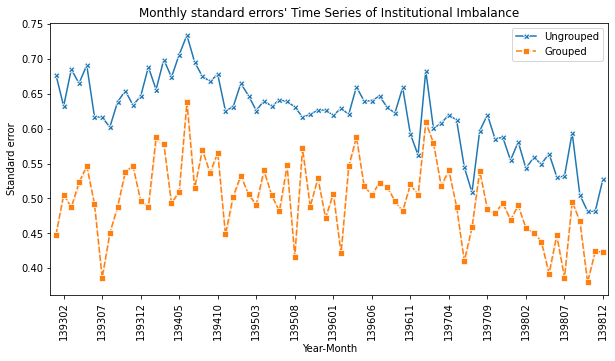
\includegraphics[width=0.85\linewidth]{Output/GroupedInsSTD.eps}
 		\label{fig:GroupedInsSTD}
 	\end{figure}
 	\begin{figure}[htbp]
 		\centering
 		\caption{text}
 		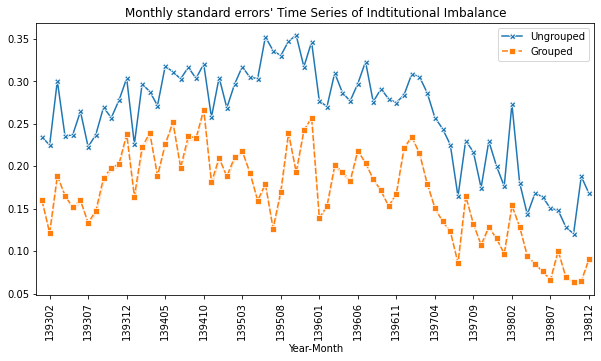
\includegraphics[width=0.85\linewidth]{Output/GroupedIndSTD.eps}
 		\label{fig:GroupedIndSTD}
 	\end{figure}
 \begin{table}[htbp]
		\centering
		\caption{text}
		\label{Imbalance}
		\resizebox{\textwidth}{!}{
			{
\def\sym#1{\ifmmode^{#1}\else\(^{#1}\)\fi}
\begin{tabular}{l*{6}{c}}
\hline\hline
                    &\multicolumn{6}{c}{Dependent Variable:  Future Pairs's Comovement}                                                                 \\\cmidrule(lr){2-7}
                    &\multicolumn{1}{c}{(1)}         &\multicolumn{1}{c}{(2)}         &\multicolumn{1}{c}{(3)}         &\multicolumn{1}{c}{(4)}         &\multicolumn{1}{c}{(5)}         &\multicolumn{1}{c}{(6)}         \\
\hline
SameGroup           &      0.0208\sym{***}&      0.0206\sym{***}&                     &                     &     0.00619         &     0.00630\sym{*}  \\
                    &      (7.91)         &      (7.94)         &                     &                     &      (1.95)         &      (2.04)         \\
[1em]
LowImbalanceStd     &                     &    -0.00144         &      0.0282\sym{***}&    -0.00724\sym{***}&    -0.00610\sym{***}&    -0.00267         \\
                    &                     &     (-1.15)         &      (6.06)         &     (-5.74)         &     (-4.87)         &     (-1.85)         \\
[1em]
 $ \text{LowImbalanceStd} \times {\text{SameGroup} } $ &                     &                     &                     &                     &      0.0358\sym{***}&      0.0325\sym{***}\\
                    &                     &                     &                     &                     &      (8.57)         &      (7.48)         \\
\hline
Sub-sample          &       Total         &       Total         &   SameGroup         &      Others         &       Total         &       Total         \\
Business Group FE   &          No         &          No         &          No         &          No         &          No         &         Yes         \\
Observations        &      354209         &      354209         &       43274         &      310935         &      354209         &      354209         \\
\hline\hline
\multicolumn{7}{l}{\footnotesize \textit{t} statistics in parentheses}\\
\multicolumn{7}{l}{\footnotesize \sym{*} \(p<0.05\), \sym{**} \(p<0.01\), \sym{***} \(p<0.001\)}\\
\end{tabular}
}

		}
	\end{table}
\FloatBarrier

 \subsection{Turnover}
\begin{table}[htbp]
				\centering
				\caption{cross-sectional average of the time-series coefficients for daily changes in turnover }
				\resizebox{0.7\textheight}{!}{
					{
\def\sym#1{\ifmmode^{#1}\else\(^{#1}\)\fi}
\begin{tabular}{l*{4}{c}}
\hline\hline
                    &\multicolumn{4}{c}{Dependent Variable: $\Delta \text{TurnOver}\_{i} $ }                 \\\cmidrule(lr){2-5}
                    &\multicolumn{1}{c}{(1)}         &\multicolumn{1}{c}{(2)}         &\multicolumn{1}{c}{(3)}         &\multicolumn{1}{c}{(4)}         \\
\hline
 $ \Delta \text{TurnOver}_{\text{Market}} $ &       0.416\sym{***}&       0.326\sym{***}&       0.252\sym{***}&       0.228\sym{***}\\
                    &     (12.25)         &      (5.35)         &      (6.41)         &      (4.24)         \\
[1em]
 $ \Delta \text{TurnOver}_{\text{Industry-i}} $ &       0.142\sym{***}&       0.213\sym{***}&      0.0335         &       0.167\sym{**} \\
                    &      (3.79)         &      (6.29)         &      (1.34)         &      (2.87)         \\
[1em]
 $ \Delta \text{TurnOver}_{\text{Group,-i}} $ &                     &                     &       0.330\sym{***}&       0.218\sym{***}\\
                    &                     &                     &     (12.74)         &      (3.80)         \\
\hline
Control             &          No         &         Yes         &          No         &         Yes         \\
Observations        &      854662         &      851772         &      333789         &      331263         \\
$ R^2 $             &       0.285         &       0.543         &       0.433         &       0.712         \\
\hline\hline
\multicolumn{5}{l}{\footnotesize \textit{t} statistics in parentheses}\\
\multicolumn{5}{l}{\footnotesize \sym{*} \(p<0.05\), \sym{**} \(p<0.01\), \sym{***} \(p<0.001\)}\\
\end{tabular}
}

				} \label{turnover}
		\end{table}
	\begin{table}[htbp]
					\centering
					\caption{cross-sectional variation in $\beta_{Group}$ }
					\resizebox{0.7\textheight}{!}{
						{
\def\sym#1{\ifmmode^{#1}\else\(^{#1}\)\fi}
\begin{tabular}{l*{14}{c}}
\hline\hline
                &\multicolumn{14}{c}{Dependent Variable: $ \beta\_{Group} $ }                                                                                                                                                                                                              \\\cmidrule(lr){2-15}
                &\multicolumn{1}{c}{(1)}         &\multicolumn{1}{c}{(2)}         &\multicolumn{1}{c}{(3)}         &\multicolumn{1}{c}{(4)}         &\multicolumn{1}{c}{(5)}         &\multicolumn{1}{c}{(6)}         &\multicolumn{1}{c}{(7)}         &\multicolumn{1}{c}{(8)}         &\multicolumn{1}{c}{(9)}         &\multicolumn{1}{c}{(10)}         &\multicolumn{1}{c}{(11)}         &\multicolumn{1}{c}{(12)}         &\multicolumn{1}{c}{(13)}         &\multicolumn{1}{c}{(14)}         \\
\hline
Excess          &    0.355\sym{***}&    0.505\sym{***}&                  &                  &                  &                  &                  &                  &                  &                  &                  &                  &                  &                  \\
                &   (4.99)         &   (6.94)         &                  &                  &                  &                  &                  &                  &                  &                  &                  &                  &                  &                  \\
[1em]
ExcessDummy     &                  &                  &  0.00604         &    0.101\sym{**} &                  &                  &                  &                  &                  &                  &                  &                  &                  &                  \\
                &                  &                  &   (0.16)         &   (2.77)         &                  &                  &                  &                  &                  &                  &                  &                  &                  &                  \\
[1em]
ExcessDiff      &                  &                  &                  &                  &    0.716\sym{***}&    0.961\sym{***}&                  &                  &                  &                  &                  &                  &                  &                  \\
                &                  &                  &                  &                  &   (5.99)         &   (7.77)         &                  &                  &                  &                  &                  &                  &                  &                  \\
[1em]
ExcessHigh      &                  &                  &                  &                  &                  &                  &    0.344\sym{***}&    0.412\sym{***}&                  &                  &                  &                  &                  &                  \\
                &                  &                  &                  &                  &                  &                  &   (6.61)         &   (8.48)         &                  &                  &                  &                  &                  &                  \\
[1em]
Low Imbalance std&                  &                  &                  &                  &                  &                  &                  &                  &  -0.0211         &   -0.144\sym{***}&                  &                  &                  &                  \\
                &                  &                  &                  &                  &                  &                  &                  &                  &  (-0.53)         &  (-3.59)         &                  &                  &                  &                  \\
[1em]
Position        &                  &                  &                  &                  &                  &                  &                  &                  &                  &                  & -0.00268         &   0.0308         &                  &                  \\
                &                  &                  &                  &                  &                  &                  &                  &                  &                  &                  &  (-0.17)         &   (1.94)         &                  &                  \\
[1em]
Centrality      &                  &                  &                  &                  &                  &                  &                  &                  &                  &                  &                  &                  &    0.397\sym{*}  &   -0.153         \\
                &                  &                  &                  &                  &                  &                  &                  &                  &                  &                  &                  &                  &   (2.47)         &  (-1.04)         \\
\hline
Observations    &     1349         &     1349         &     1367         &     1367         &     1349         &     1349         &     1367         &     1367         &     1341         &     1341         &     1349         &     1349         &     1299         &     1299         \\
Time FE         &      Yes         &      Yes         &      Yes         &      Yes         &      Yes         &      Yes         &      Yes         &      Yes         &      Yes         &      Yes         &      Yes         &      Yes         &      Yes         &      Yes         \\
Controls        &       No         &      Yes         &       No         &      Yes         &       No         &      Yes         &       No         &      Yes         &       No         &      Yes         &       No         &      Yes         &       No         &      Yes         \\
$ R^2 $         &   0.0251         &   0.0970         & 0.000973         &   0.0600         &   0.0436         &    0.123         &   0.0436         &    0.109         &  0.00130         &   0.0640         &  0.00128         &   0.0581         &  0.00415         &   0.0456         \\
\hline\hline
\multicolumn{15}{l}{\footnotesize \textit{t} statistics in parentheses}\\
\multicolumn{15}{l}{\footnotesize \sym{*} \(p<0.05\), \sym{**} \(p<0.01\), \sym{***} \(p<0.001\)}\\
\end{tabular}
}

					}
				 \label{Turnovercrosssection}
			\end{table}


\begin{table}[htbp]
				\centering
				\caption{Pairwise correlation in turnover  }
				\label{mresult2-turnover}
				\resizebox{0.7\textheight}{!}{
					\centering
					{
\def\sym#1{\ifmmode^{#1}\else\(^{#1}\)\fi}
\begin{tabular}{l*{7}{c}}
\hline\hline
                    &\multicolumn{7}{c}{Dependent Variable:  Monthly Correlation of Delta turnover}                                                                           \\\cmidrule(lr){2-8}
                    &\multicolumn{1}{c}{(1)}         &\multicolumn{1}{c}{(2)}         &\multicolumn{1}{c}{(3)}         &\multicolumn{1}{c}{(4)}         &\multicolumn{1}{c}{(5)}         &\multicolumn{1}{c}{(6)}         &\multicolumn{1}{c}{(7)}         \\
\hline
SameGroup           &      0.0180\sym{***}&                     &      0.0173\sym{***}&                     &                     &      0.0150\sym{***}&      0.0168\sym{***}\\
                    &      (6.19)         &                     &      (5.53)         &                     &                     &      (4.89)         &      (5.40)         \\
[1em]
$ \text{MFCAP*} $   &                     &     0.00219\sym{**} &    0.000543         &     0.00115         &    0.000372         &    0.000363         &   -0.000413         \\
                    &                     &      (2.84)         &      (0.69)         &      (0.57)         &      (0.41)         &      (0.40)         &     (-0.37)         \\
[1em]
 $ (\text{MFCAP}^*) \times {\text{SameGroup} }  $ &                     &                     &                     &                     &                     &     0.00260         &     0.00296         \\
                    &                     &                     &                     &                     &                     &      (1.03)         &      (1.19)         \\
\hline
Sub-sample          &         All         &         All         &         All         &   SameGroup         &      Others         &         All         &         All         \\
Business Group FE   &          No         &          No         &          No         &          No         &          No         &          No         &         Yes         \\
Observations        &      294864         &      294864         &      294864         &       37076         &      257788         &      294864         &      294864         \\
\hline\hline
\multicolumn{8}{l}{\footnotesize \textit{t} statistics in parentheses}\\
\multicolumn{8}{l}{\footnotesize \sym{*} \(p<0.05\), \sym{**} \(p<0.01\), \sym{***} \(p<0.001\)}\\
\end{tabular}
}

				}
		\end{table}

\FloatBarrier


 \subsection{Big business group}
		\begin{table}[htbp]
				\centering
				\caption{heading}
				\label{BigBusinessGroup}
				\resizebox{\textwidth}{!}{
					{
\def\sym#1{\ifmmode^{#1}\else\(^{#1}\)\fi}
\begin{tabular}{l*{5}{c}}
\hline\hline
                &\multicolumn{5}{c}{Dependent Variable: Future Pairs's co-movement}                            \\\cmidrule(lr){2-6}
                &\multicolumn{1}{c}{(1)}         &\multicolumn{1}{c}{(2)}         &\multicolumn{1}{c}{(3)}         &\multicolumn{1}{c}{(4)}         &\multicolumn{1}{c}{(5)}         \\
\hline
Same Group      &   0.0263\sym{***}&   0.0250\sym{***}&   0.0380\sym{***}&   0.0244\sym{**} &   0.0256\sym{***}\\
                &   (3.79)         &   (3.55)         &   (5.82)         &   (3.33)         &   (4.02)         \\
[1em]
 $ {\rho\_t(\text{Turnover})} $ &  0.00475\sym{***}&  0.00419\sym{***}&  0.00474\sym{***}&  0.00383\sym{***}&  0.00493\sym{***}\\
                &   (9.75)         &   (8.55)         &   (4.65)         &   (4.64)         &   (4.66)         \\
[1em]
 $ {\rho\_t} $   &   0.0249\sym{***}&   0.0248\sym{***}&   0.0248\sym{***}&   0.0252\sym{***}&   0.0243\sym{***}\\
                &  (11.12)         &  (11.10)         &  (11.03)         &  (10.64)         &   (8.58)         \\
[1em]
$ {\text{SameGroup} \times  {\rho\_t(\text{Turnover})} } $ &                  &   0.0172\sym{***}& -0.00936         &   0.0224\sym{***}&  -0.0114         \\
                &                  &   (3.63)         &  (-0.84)         &   (4.42)         &  (-1.04)         \\
[1em]
BigGroup        &                  &                  & -0.00186         &                  &                  \\
                &                  &                  &  (-1.99)         &                  &                  \\
[1em]
$ {\text{BigGroup} } \times {\text{SameGroup} }  $ &                  &                  &  -0.0151\sym{*}  &                  &                  \\
                &                  &                  &  (-2.43)         &                  &                  \\
[1em]
$ {\text{BigGroup} } \times  {\rho\_t(\text{Turnover})}  $ &                  &                  &-0.000833         &                  &                  \\
                &                  &                  &  (-0.53)         &                  &                  \\
[1em]
$ {\text{BigGroup}}\times{\text{SameGroup}}\times  {\rho\_t(\text{Turnover})}$ &                  &                  &   0.0317\sym{*}  &                  &                  \\
                &                  &                  &   (2.64)         &                  &                  \\
\hline
Observations    &  1459585         &  1459585         &  1459585         &   957316         &   502269         \\
Controls        &      Yes         &      Yes         &      Yes         &      Yes         &      Yes         \\
Pari Size FE    &      Yes         &      Yes         &      Yes         &      Yes         &      Yes         \\
SubSample       &      All         &      All         &      All         &Big Groups         &   Others         \\
$ R^2$          &  0.00244         &  0.00255         &  0.00302         &  0.00307         &  0.00396         \\
\hline\hline
\multicolumn{6}{l}{\footnotesize \textit{t} statistics in parentheses}\\
\multicolumn{6}{l}{\footnotesize \sym{*} \(p<0.05\), \sym{**} \(p<0.01\), \sym{***} \(p<0.001\)}\\
\end{tabular}
}

				}
		\end{table}

\section{Conclusion}


\newpage


\footnotesize{
	\bibliographystyle{apalike}
	\bibliography{Ref}
}



\end{document}